% This file was created with tikzplotlib v0.10.1.
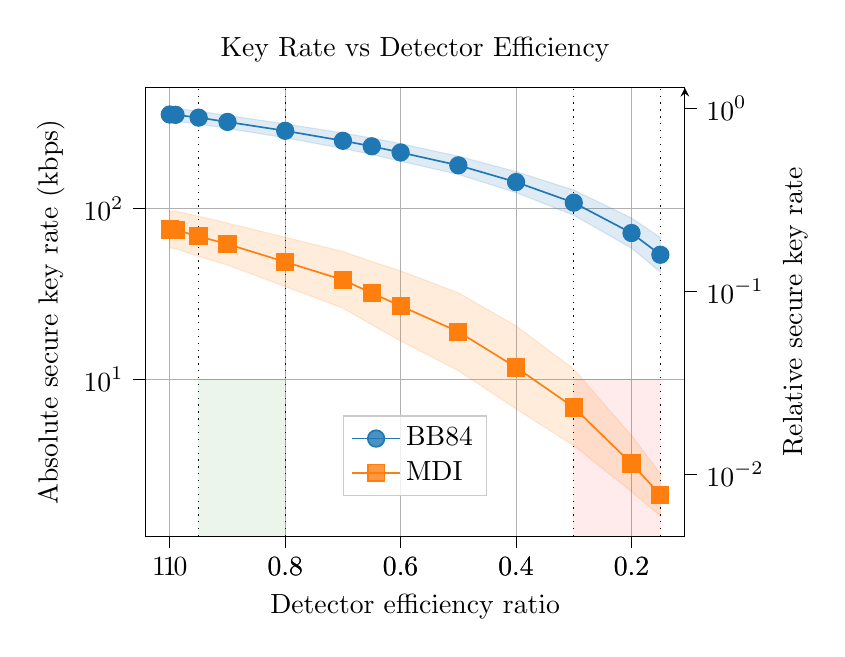
\begin{tikzpicture}
\definecolor{darkgray176}{RGB}{176,176,176}
\definecolor{darkgreen}{RGB}{0,100,0}
\definecolor{darkorange25512714}{RGB}{255,127,14}
\definecolor{darkred}{RGB}{139,0,0}
\definecolor{dimgray}{RGB}{105,105,105}
\definecolor{green}{RGB}{0,128,0}
\definecolor{lightgray204}{RGB}{204,204,204}
\definecolor{steelblue31119180}{RGB}{31,119,180}
\begin{axis}[
legend cell align={left},
legend style={
  fill opacity=0.8,
  draw opacity=1,
  text opacity=1,
  at={(0.5,0.09)},
  anchor=south,
  draw=lightgray204
},
log basis y={10},
tick align=outside,
tick pos=left,
x dir=reverse,
x grid style={darkgray176},
xlabel={Detector efficiency ratio},
xmajorgrids,
xmin=0.1075, xmax=1.0425,
xtick style={color=black},
xtick={0,0.2,0.4,0.6,0.8,1,1.2},
xticklabels={
  \(\displaystyle {0.0}\),
  \(\displaystyle {0.2}\),
  \(\displaystyle {0.4}\),
  \(\displaystyle {0.6}\),
  \(\displaystyle {0.8}\),
  \(\displaystyle {1.0}\),
  \(\displaystyle {1.2}\)
},
y grid style={darkgray176},
ylabel={Absolute secure key rate (kbps)},
ymajorgrids,
ymin=1.2053868575152, ymax=509.443108388431,
ymode=log,
ytick style={color=black},
ytick={0.1,1,10,100,1000,10000},
yticklabels={
  \(\displaystyle {10^{-1}}\),
  \(\displaystyle {10^{0}}\),
  \(\displaystyle {10^{1}}\),
  \(\displaystyle {10^{2}}\),
  \(\displaystyle {10^{3}}\),
  \(\displaystyle {10^{4}}\)
}
]
\path [draw=green, fill=green, opacity=0.08]
(axis cs:0.8,0)
--(axis cs:0.8,1)
--(axis cs:0.95,1)
--(axis cs:0.95,0)
--cycle;
\path [draw=red, fill=red, opacity=0.08]
(axis cs:0.15,0)
--(axis cs:0.15,1)
--(axis cs:0.3,1)
--(axis cs:0.3,0)
--cycle;
\path [draw=steelblue31119180, fill=steelblue31119180, opacity=0.15]
(axis cs:1,387.020039953177)
--(axis cs:1,326.784941325102)
--(axis cs:0.99,325.001568723552)
--(axis cs:0.95,312.892198589077)
--(axis cs:0.9,294.683566105314)
--(axis cs:0.8,260.016804432527)
--(axis cs:0.7,224.830369730963)
--(axis cs:0.65,207.407342778991)
--(axis cs:0.6,189.342751187773)
--(axis cs:0.5,158.577299581162)
--(axis cs:0.4,124.132245071418)
--(axis cs:0.3,91.3490986724699)
--(axis cs:0.2,58.7229160576156)
--(axis cs:0.15,42.5240343359016)
--(axis cs:0.15,67.6780421922832)
--(axis cs:0.15,67.6780421922832)
--(axis cs:0.2,88.0875011344346)
--(axis cs:0.3,128.377542982802)
--(axis cs:0.4,164.715882114328)
--(axis cs:0.5,202.637612195008)
--(axis cs:0.6,240.007489693741)
--(axis cs:0.65,258.984528392764)
--(axis cs:0.7,277.026965695373)
--(axis cs:0.8,313.604420826316)
--(axis cs:0.9,351.508611355208)
--(axis cs:0.95,371.787360943714)
--(axis cs:0.99,386.091494303437)
--(axis cs:1,387.020039953177)
--cycle;
\path [draw=darkorange25512714, fill=darkorange25512714, opacity=0.15]
(axis cs:1,96.6582415105608)
--(axis cs:1,58.8626395092792)
--(axis cs:0.99,58.2663143626435)
--(axis cs:0.95,52.4550196355945)
--(axis cs:0.9,46.7118847307108)
--(axis cs:0.8,34.9403671571846)
--(axis cs:0.7,26.1126238451336)
--(axis cs:0.65,20.8949626643841)
--(axis cs:0.6,16.7653131495295)
--(axis cs:0.5,11.2455587299253)
--(axis cs:0.4,6.71067406086006)
--(axis cs:0.3,4.08740249104616)
--(axis cs:0.2,2.19754216364582)
--(axis cs:0.15,1.58667759834194)
--(axis cs:0.15,2.80547764374813)
--(axis cs:0.15,2.80547764374813)
--(axis cs:0.2,4.68185069496077)
--(axis cs:0.3,11.4728834713094)
--(axis cs:0.4,20.5606290909527)
--(axis cs:0.5,32.1012746574682)
--(axis cs:0.6,43.1574614370099)
--(axis cs:0.65,48.9785154444466)
--(axis cs:0.7,56.0490452647734)
--(axis cs:0.8,67.8878192990638)
--(axis cs:0.9,82.2558623684844)
--(axis cs:0.95,90.1358714977511)
--(axis cs:0.99,96.6723693238148)
--(axis cs:1,96.6582415105608)
--cycle;
\addplot [semithick, steelblue31119180, mark=*, mark size=3, mark options={solid}]
table {%
1 355.629471568004
0.99 354.232044455943
0.95 341.070908717395
0.9 321.844389590497
0.8 285.55633307488
0.7 249.567776611359
0.65 231.765598946033
0.6 213.175229340287
0.5 179.258822197009
0.4 142.991441162647
0.3 108.292071922488
0.2 71.9218668753984
0.15 53.6464667053782
};
\addlegendentry{BB84}
\addplot [semithick, darkorange25512714, mark=square*, mark size=3, mark options={solid}]
table {%
1 75.4291669424831
0.99 75.0515999909594
0.95 68.7610275467576
0.9 61.9865014449264
0.8 48.7034427100374
0.7 38.2568639054209
0.65 31.9906900764687
0.6 26.8988541713251
0.5 18.9999149857578
0.4 11.7463049643546
0.3 6.84794074741542
0.2 3.20757919716268
0.15 2.10983139847341
};
\addlegendentry{MDI}
\addplot [line width=0.48pt, black, dotted, forget plot]
table {%
0.8 1.2053868575152
0.8 509.443108388431
};
\addplot [line width=0.48pt, black, dotted, forget plot]
table {%
0.95 1.2053868575152
0.95 509.443108388431
};
\addplot [line width=0.48pt, black, dotted, forget plot]
table {%
0.15 1.2053868575152
0.15 509.443108388431
};
\addplot [line width=0.48pt, black, dotted, forget plot]
table {%
0.3 1.2053868575152
0.3 509.443108388431
};
\draw (axis cs:0.96122,0.01) node[
  scale=0.35,
  anchor=south east,
  text=dimgray,
  rotate=0.0
]{0.95};
\draw (axis cs:0.13878,0.01) node[
  scale=0.35,
  anchor=south west,
  text=dimgray,
  rotate=0.0
]{0.15};
\draw (axis cs:0.31122,0.01) node[
  scale=0.35,
  anchor=south east,
  text=dimgray,
  rotate=0.0
]{0.30};
\draw (axis cs:0.875,0.97) node[
  scale=0.35,
  anchor=north,
  text=darkgreen,
  rotate=0.0
]{\itshape SNSPD};
\draw (axis cs:0.225,0.97) node[
  scale=0.35,
  anchor=north,
  text=darkred,
  rotate=0.0
]{\itshape InGaAs SPAD};
\end{axis}
\begin{axis}[
axis y line=right,
log basis y={10},
tick align=outside,
title={Key Rate vs Detector Efficiency},
x dir=reverse,
x grid style={darkgray176},
xmin=0.1075, xmax=1.0425,
xtick pos=left,
xtick style={color=black},
y grid style={darkgray176},
ylabel={Relative secure key rate},
ymin=0.00459105512184768, ymax=1.29222309811562,
ymode=log,
ytick pos=right,
ytick style={color=black},
ytick={0.0001,0.001,0.01,0.1,1,10,100},
yticklabel style={anchor=west},
yticklabels={
  \(\displaystyle {10^{-4}}\),
  \(\displaystyle {10^{-3}}\),
  \(\displaystyle {10^{-2}}\),
  \(\displaystyle {10^{-1}}\),
  \(\displaystyle {10^{0}}\),
  \(\displaystyle {10^{1}}\),
  \(\displaystyle {10^{2}}\)
}
]
\addplot [semithick, steelblue31119180, opacity=0, mark=*, mark size=3, mark options={solid}]
table {%
1 1
0.99 0.996070553135264
0.95 0.959062552418901
0.9 0.90499920653779
0.8 0.802960260340167
0.7 0.701763482961611
0.65 0.65170526482003
0.6 0.599430717595978
0.5 0.504060648873223
0.4 0.402079840380449
0.3 0.304508148452989
0.2 0.202238207531811
0.15 0.150849327725416
};
\addplot [semithick, darkorange25512714, opacity=0, mark=square*, mark size=3, mark options={solid}]
table {%
1 0.212100438723227
0.99 0.21103875238475
0.95 0.193350194638211
0.9 0.17430080013229
0.8 0.136949962260718
0.7 0.10757506608421
0.65 0.0899551151804678
0.6 0.0756373032097861
0.5 0.0534261541991594
0.4 0.0330296162254608
0.3 0.0192558302809444
0.2 0.00901944145129525
0.15 0.00593266747317361
};
\end{axis}
\end{tikzpicture}
